\documentclass[runningheads]{llncs}

\usepackage{cite}
\usepackage{graphicx}
\usepackage{amsmath,amssymb,amsfonts}
\usepackage{textcomp}
\usepackage{xcolor}
\usepackage{booktabs}
\usepackage{array}
\usepackage{url}
\usepackage{hyperref}
\usepackage{tikz}
\usepackage{pgfplots}
\usepackage{comment}
\pgfplotsset{compat=1.18}
\usetikzlibrary{shapes.geometric,arrows.meta,positioning,fit,backgrounds,calc}

\hypersetup{colorlinks=true,linkcolor=blue,citecolor=blue,urlcolor=blue}

% ---- TikZ style definitions ----
\tikzset{
  pbox/.style={draw, rounded corners=3pt, minimum width=1.55cm,
               minimum height=0.50cm, font=\scriptsize\bfseries,
               align=center, fill=#1!15, draw=#1!55!black},
  pbox/.default=blue,
  parr/.style={-{Stealth[length=3.5pt]}, thick, gray!65!black},
  skarr/.style={parr, dashed, gray!50},
  grp/.style={draw=gray!45, rounded corners=4pt, dashed,
              inner sep=3.5pt, fill=gray!6},
}

\begin{document}

\title{Explainable Ensemble Framework for Cross-Dataset Cervical Cytology with Bethesda System Mapping}
\titlerunning{Explainable Ensemble Framework for Cervical Cytology}

% NOTE: confirm the spelling of the first author's surname
% ("Srivatsava" vs. "Srivastava") before submission.
\author{Devanshi Srivatsava\inst{1} \and
Kumar Satyam\inst{1} \and
Tanisha D Jogi\inst{1} \and
Natarajan Venkateswaran\inst{1} \and
Sumathi.D\inst{1} \and
T.Poongodi\inst{1}}

\authorrunning{D. Srivatsava et al.}

\institute{Department of Computer Science Engineering,\\
Dayananda Sagar University, Bangalore, India\\
\email{natarajanv25@gmail.com, srivdevanshi@gmail.com, satyamraj54671@gmail.com, tanishajogi551@gmail.com, sumathi.research28@gmail.com, tpoongodi2730@gmail.com}}

\maketitle

%------------------------------------------------------------------
\begin{abstract}
Cervical cancer accounts for nearly 340,000 deaths annually worldwide, and a large share of these occur in regions with a severe shortage of experienced cytopathologists. Although Pap smear screening is effective in principle, its sensitivity varies widely in practice, depending largely on the skill and fatigue of the reader. This work presents an automatic classification system built on three deep learning backbones --- ResNet50, EfficientNet-B0, and Swin Transformer --- and a soft-voting ensemble of all three, trained and tested on the union of the SIPaKMeD (five categories, 4,049 cells) and Herlev (seven categories, 917 cells) datasets. Both binary (Normal vs.\ Abnormal) and multiclass classification are investigated. Among the individual networks, Swin Transformer performs best, with a multiclass accuracy of 96.8\% and a macro area under the receiver operating characteristic curve (ROC-AUC) of 0.987; the three-model ensemble reaches 97.1\%. Models trained on one dataset and tested on the other drop to 68--80\% accuracy, which quantifies the domain gap between the two sources; training on the combined data yields 88--96\% on the held-out portion of each source, an in-distribution result. Because the split is made at the cell-image level, these in-distribution figures may be optimistic. Grad-CAM++ is integrated into the inference process to provide a visual explanation of each prediction by highlighting the image regions that drive it.

\keywords{Cervical cancer \and Pap smear \and Deep learning \and EfficientNet-B0 \and ResNet50 \and Swin Transformer \and Grad-CAM++ \and Explainable AI \and SIPaKMeD \and Herlev \and Multiclass classification \and U-Net \and Segmentation \and Bethesda System}
\end{abstract}

%------------------------------------------------------------------
\section{Introduction}

The peculiar paradox of cervical cancer is that, although a vaccine, a reasonably good screening tool, and a clear understanding of its development through high-risk HPV infection are all available, mortality rates in low-income countries have not changed over the past two decades \cite{who2022}. The problem is largely one of access, and a key bottleneck is the availability of trained pathologists. Where organized screening programs staffed by experienced cytologists exist, the five-year survival rate in developed countries approaches 90\% \cite{arbyn2010}.

Pap smear interpretation demands expertise, repetition, and sustained concentration. Inter-observer agreement on difficult samples can be poor, and fatigue is common. Automated image analysis has been pursued for decades as a way to extend scarce human resources; yet most studies focus on a single dataset, omit any explainability component, or validate performance on a small hold-out set. This paper attempts to address these issues together.

Our specific contributions are: (1) a comparison of three architecturally different networks --- ResNet50 \cite{he2016deep}, EfficientNet-B0 \cite{tan2019efficientnet}, and Swin Transformer \cite{liu2021swin} --- and their soft-voting ensemble on both binary and multiclass classification; (2) a cross-dataset study in which models trained on SIPaKMeD \cite{plissiti2018sipakmed} are tested on Herlev \cite{jantzen2005} and vice versa; (3) a U-Net-based nuclear segmentation stage applied before classification; (4) a mapping of model outputs to Bethesda-oriented categories; and (5) the integration of Grad-CAM++ \cite{chattopadhay2018} into an explainable dashboard prototype.

%------------------------------------------------------------------
\section{Related Work}

Early computational approaches to cervical cytology relied on handcrafted morphological features --- nuclear area, elongation, Haralick texture statistics --- fed into SVM or $k$-NN classifiers. Jantzen et al.\ \cite{jantzen2005} introduced the Herlev benchmark to evaluate such approaches and reported reasonable two-class accuracy, although the features required careful tuning to the staining protocol in use.

CNN-based methods marked a turning point, and fine-tuning ImageNet-pretrained backbones quickly became the standard strategy. Zhang et al.\ \cite{zhang2017deeppap} fine-tuned a pretrained ConvNet to classify cervical cells directly, without prior segmentation, and evaluated it on Herlev with five-fold cross-validation. Lin et al.\ \cite{lin2019} combined cell appearance with cell morphology as joint CNN inputs and evaluated on Herlev using five-fold cross-validation with patient-level splitting, which is the evaluation design needed to avoid leakage between training and test cells. Rahaman et al.\ \cite{rahaman2020} survey deep learning for cervical cytopathology image analysis more broadly. More recently, the Swin Transformer \cite{liu2021swin} has shown that hierarchical windowed attention performs strongly in computational pathology, and hierarchical vision transformers have been scaled to gigapixel whole-slide images \cite{chen2022hipt}.

Several recent developments are directly relevant to this work. The CRIC Cervix collection \cite{rezende2021cric} provides 400 conventional Pap smear images with 11,534 cells labelled by cytopathologists according to the Bethesda System, offering native Bethesda ground truth that SIPaKMeD and Herlev lack. HiCervix \cite{cai2024hicervix} extends this to 40,229 cells organized in a three-level hierarchy and benchmarks a hierarchical Swin-based classifier. Hybrid CNN--transformer designs have also appeared: CVM-Cervix \cite{liu2022cvmcervix} fuses CNN and vision-transformer features through a multilayer perceptron and was trained on combined SIPaKMeD and CRIC data, and MaxCerVixT \cite{pacal2024maxcervixt} proposes a lightweight vision transformer for cervical cytology classification.

Explainability has tended to trail raw performance gains in the cervical cytology literature. Grad-CAM \cite{selvaraju2017gradcam} and its successor Grad-CAM++ \cite{chattopadhay2018} have been used in dermatology \cite{esteva2017} and radiology \cite{rajpurkar2017}, but rigorous validation against established cytopathological criteria in cervical cell images remains limited. Cross-dataset generalization has likewise received little direct study in cervical cytology. In histopathology, Stacke et al.\ \cite{stacke2021domainshift} quantified how differences in staining and scanning between sites produce domain shift that degrades model performance on unseen data. This observation motivated both the single-source transfer experiments and the multi-dataset training reported here.

In summary, most prior studies use a single dataset or a single architecture, or provide no interpretability. The present work evaluates three backbones and their ensemble on SIPaKMeD and Herlev, measures single-source cross-dataset transfer explicitly, applies a U-Net nuclear segmentation stage before classification, maps outputs to Bethesda-oriented categories, and attaches a Grad-CAM++ explanation to each prediction.

%------------------------------------------------------------------
\section{Methodology}
\label{sec:method}

\subsection{Dataset Description}
\label{sec:data}

Two open-access databases, SIPaKMeD \cite{plissiti2018sipakmed} and Herlev \cite{jantzen2005}, were used in this study. SIPaKMeD contains 4,049 single-cell images, cropped from 966 multi-cell Pap smear images, in five groups: Superficial-Intermediate, Parabasal, Koilocytotic, Dyskeratotic, and Metaplastic. Koilocytotic and Dyskeratotic cells correspond to pre-cancerous states. Herlev comprises 917 single-cell images in seven categories ranging from normal cells to carcinoma in situ.

Because the two databases were acquired with different staining and imaging procedures, combining them exposes the models to a wider range of appearance. Classes were harmonized according to their cytological similarity. For binary classification, the SIPaKMeD Superficial-Intermediate and Metaplastic classes and the three Herlev normal classes are labelled Normal, and all remaining classes are labelled Abnormal (Table~\ref{tab:bethesda}).

After harmonization, 4,966 images are available. They are divided into training, validation, and test subsets in a 70:15:15 ratio by stratified sampling (Table~\ref{tab:dataset}), which preserves class proportions across the three subsets. A fixed random seed of 42 was used for all splits, and the same split and class-harmonization rules were used in every experiment reported in this paper. No source-specific duplicate removal was applied. The training subset is used to fit model parameters and to estimate normalization statistics, the validation subset for model selection and early stopping, and the test subset only for final performance reporting.

\textit{Split granularity.} The split is made at the level of individual cell images. Stratified sampling preserves class balance but does not prevent cells cropped from the same SIPaKMeD source image (or, in Herlev, from the same slide) from appearing in both the training and test subsets; Herlev does not provide patient or slide identifiers that would allow a grouped split. Cells from the same field share staining and acquisition conditions, so the in-distribution results in Tables~\ref{tab:multiclass}, \ref{tab:binary}, and~\ref{tab:cross} may be optimistic relative to a patient- or slide-level split such as that used by Lin et al.\ \cite{lin2019}. A grouped split on SIPaKMeD source images is planned as future work (Section~\ref{sec:conclusion}).

\begin{table}[t]
\caption{Combined Dataset After Harmonization}
\label{tab:dataset}
\centering
\begin{tabular}{lcc}
\toprule
\textbf{Source} & \textbf{Classes} & \textbf{Images}\\
\midrule
SIPaKMeD & 5 & 4,049\\
Herlev   & 7 & 917\\
\midrule
\textbf{Combined} & \textbf{7} & \textbf{4,966}\\
\quad Training (70\%) & --- & 3,476\\
\quad Validation (15\%) & --- & 745\\
\quad Test (15\%) & --- & 745\\
\bottomrule
\end{tabular}
\end{table}

\subsection{Preprocessing}
\label{sec:preproc}

Each image is resized to $224\times224$ pixels to match the input size of the networks. Normalization is applied per channel, using the mean and standard deviation of each channel computed on the training split:
\begin{equation}
    \hat{x}_c = \frac{x_c - \mu_c}{\sigma_c}, \quad c \in \{R,G,B\}
    \label{eq:norm}
\end{equation}
where $x_c$ denotes the original pixel intensity in color channel $c$, $\mu_c$ is the mean pixel intensity for channel $c$ computed from the training split, $\sigma_c$ is the corresponding standard deviation, and $\hat{x}_c$ is the normalized pixel intensity. The channel index $c\in\{R,G,B\}$ refers to the red, green, and blue channels. The statistics estimated on the training split are applied unchanged to the validation and test images.

Several augmentations are used to improve generalization. Because cell orientation is arbitrary, random rotations of up to 30 degrees are applied together with horizontal and vertical flips, each with probability 0.5. To simulate variation in staining, color jittering is applied to brightness, contrast, saturation, and hue.

MixUp \cite{zhang2018mixup} is also performed at the batch level, blending two images and their labels by a weighted average:
\begin{equation}
    \tilde{x}=\lambda x_i+(1{-}\lambda)x_j,\quad
    \tilde{y}=\lambda y_i+(1{-}\lambda)y_j,\quad
    \lambda\sim\mathrm{Beta}(0.4,0.4)
    \label{eq:mixup}
\end{equation}
where $x_i$ and $x_j$ denote the two input images selected for mixing, $y_i$ and $y_j$ denote their one-hot labels, $\lambda$ is the mixing coefficient sampled from a Beta distribution with parameters $(0.4,0.4)$, and $\tilde{x}$ and $\tilde{y}$ denote the resulting mixed image and mixed label. The complementary coefficient $(1-\lambda)$ determines the contribution of the second sample, so the mixed target retains contributions from both samples. This encourages smoother decision boundaries.

Weighted sampling is used to address class imbalance, with class weights $w_k = N/(K\cdot n_k)$, where $N$ is the number of training samples, $K$ is the number of classes, and $n_k$ is the number of training samples in class $k$. The weight $w_k$ increases the relative contribution of under-represented classes. Augmentation and weighted sampling are applied to the training split only; validation and test images are not augmented.

\subsection{U-Net Based Segmentation}
\label{sec:unet}

To focus the classifiers on cellular structure rather than background, a U-Net \cite{ronneberger2015unet} segmentation stage is applied to the Pap smear cell images before classification. U-Net is a convolutional encoder--decoder architecture with skip connections, designed for biomedical image segmentation. During encoding, the network extracts features such as nuclear boundaries, chromatin texture, and perinuclear morphology; the decoder recovers a spatial nuclear mask.

\begin{figure}[t]
\centering
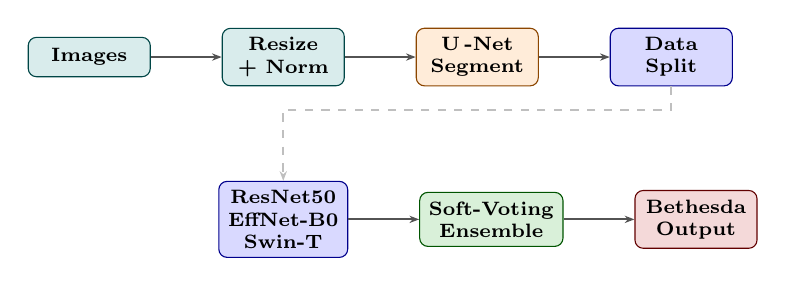
\begin{tikzpicture}[
    node distance=0.7cm and 0.9cm,
    every node/.style={align=center, font=\small}
]
  %% ---- preprocessing ----
  \node[pbox=teal]  (raw) {Images};
  \node[pbox=teal, right=of raw] (pre) {Resize\\+ Norm};
  \node[pbox=orange, right=of pre] (seg) {U\,-Net\\Segment};
  \node[pbox=blue, right=of seg] (spl) {Data\\Split};
  \draw[parr](raw)--(pre);
  \draw[parr](pre)--(seg);
  \draw[parr](seg)--(spl);
  %% ---- models ----
  \node[pbox=blue, below=1.2cm of pre] (mdl) {ResNet50\\EffNet-B0\\Swin-T};
  \node[pbox=green!60!black, right=of mdl] (ens) {Soft-Voting\\Ensemble};
  \node[pbox=red!70!black, right=of ens] (out) {Bethesda\\Output};
  \draw[parr](mdl)--(ens);
  \draw[parr](ens)--(out);
  \draw[skarr](spl.south)--++(0,-0.3)-|(mdl.north);
\end{tikzpicture}
\caption{Overall system model: image preprocessing, U-Net nuclear segmentation, classification by three backbones, soft-voting ensemble of all three (Eq.~\ref{eq:ensemble}), and Bethesda-oriented output mapping.}
\label{fig:pipeline}
\end{figure}

Figure~\ref{fig:pipeline} summarizes the processing flow. Input cell images are resized and normalized before segmentation, and the segmented images are passed to the classification backbones. ResNet50, EfficientNet-B0, and Swin Transformer are evaluated as individual models, and the ensemble combines the class probabilities of all three by the soft-voting rule in Eq.~\ref{eq:ensemble}. The final output is presented with a Bethesda-oriented interpretation and a Grad-CAM++ explanation. Dataset splitting is performed for model evaluation, and augmentation is restricted to the training data.

% ---- U-Net Architecture ----
\begin{figure}[t]
\centering
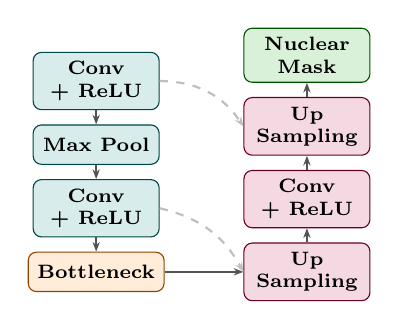
\begin{tikzpicture}[node distance=0.18cm and 0.2cm]

  %% ---- Encoder ----
  \node[pbox=teal, minimum width=1.6cm]  (e1) {Conv\\+ ReLU};
  \node[pbox=teal, below=of e1, minimum width=1.6cm] (e2) {Max Pool};
  \node[pbox=teal, below=of e2, minimum width=1.6cm] (e3) {Conv\\+ ReLU};
  \node[pbox=orange, below=of e3, minimum width=1.6cm] (bot) {Bottleneck};

  \draw[parr](e1)--(e2);
  \draw[parr](e2)--(e3);
  \draw[parr](e3)--(bot);

  %% ---- Decoder ----
  \node[pbox=purple, minimum width=1.6cm, right=1cm of bot] (d1) {Up\\Sampling};
  \node[pbox=purple, above=of d1, minimum width=1.6cm] (d2) {Conv\\+ ReLU};
  \node[pbox=purple, above=of d2, minimum width=1.6cm] (d3) {Up\\Sampling};
  \node[pbox=green!60!black, above=of d3, minimum width=1.6cm] (out) {Nuclear\\Mask};

  \draw[parr](bot)--(d1);
  \draw[parr](d1)--(d2);
  \draw[parr](d2)--(d3);
  \draw[parr](d3)--(out);

  %% ---- Skip connections ----
  \draw[skarr, thick, bend left=28](e1.east) to (d3.west);
  \draw[skarr, thick, bend left=24](e3.east) to (d1.west);

\end{tikzpicture}

\caption{Encoder--decoder structure of the U-Net used for nuclear segmentation. Skip connections transfer spatial details from the encoder to the decoder.}
\label{fig:unet}
\end{figure}

Figure~\ref{fig:unet} illustrates the encoder--decoder path. The encoder progressively extracts features while reducing spatial resolution, the bottleneck holds the most compressed representation, and the decoder upsamples these features to recover a spatial mask. Skip connections combine encoder details with decoder features to preserve boundary information, integrating high-level semantic information with fine-grained localization cues.

The U-Net is trained on the MoNuSeg dataset \cite{kumar2017monuseg}, which provides expert-annotated nuclear masks from H\&E-stained histopathology tissue, and is then applied without fine-tuning to the Papanicolaou-stained cytology images of SIPaKMeD and Herlev. This is a transfer across both stain and specimen type. Segmentation quality on the cervical images was not quantified: no Dice score or other overlap measure is reported, although both SIPaKMeD and Herlev provide nucleus annotations that would permit such an evaluation. The contribution of the segmentation stage to classification accuracy was also not isolated by an ablation. The segmentation stage should therefore be regarded as a pre-processing step whose effect is untested, and its evaluation is listed as a limitation.

\subsection{Feature Extraction and Classification}

Three deep learning architectures are evaluated: ResNet50, EfficientNet-B0, and Swin Transformer. The segmented cell images produced by the U-Net stage are passed as inputs to each backbone. The architectures are described in Section~\ref{sec:archs}.

\subsection{Bethesda System Mapping}
\label{sec:bethesda}

SIPaKMeD and Herlev use different class definitions and naming conventions, which complicates direct comparison and cross-dataset evaluation. To provide a common clinical frame of reference, the dataset-specific classes were mapped to categories oriented to the Bethesda System for Reporting Cervical Cytology (TBS), the internationally recognized standard for cervical cytology reporting.

The first level is the binary Normal/Abnormal distinction. Within TBS, abnormal squamous findings are further divided into Atypical Squamous Cells of Undetermined Significance (ASC-US), Low-grade Squamous Intraepithelial Lesions (LSIL), and High-grade Squamous Intraepithelial Lesions (HSIL). ASC-US denotes changes that are suggestive of, but insufficient for, a lesion; LSIL reflects early HPV-induced changes; and HSIL represents moderate to severe abnormalities with a higher risk of progression to cancer.

Neither SIPaKMeD nor Herlev includes Bethesda labels, so dataset classes were assigned to Bethesda-oriented categories by morphological correspondence. Koilocytotic cells (SIPaKMeD) and mild dysplasia (Herlev) were assigned to LSIL, and severe dysplasia and carcinoma in situ (Herlev) were assigned to HSIL. Table~\ref{tab:bethesda} lists the mapping.

In the deployed dashboard, the reported category is obtained from a fused clinical score $S \in [0,1]$ that combines the ensemble output with three groups of handcrafted cytological features:
\begin{equation}
    S = 0.4\,c_{\text{model}} + 0.2\,s_{\text{nuc}} + 0.3\,s_{\text{cyto}} + 0.1\,s_{\text{bg}},
    \label{eq:fusion}
\end{equation}
where $c_{\text{model}}$ is the maximum class probability of the classifier and $s_{\text{nuc}}$, $s_{\text{cyto}}$, and $s_{\text{bg}}$ are the overall nuclear, cytoplasmic, and background feature scores. The score is assigned to a TBS category by fixed intervals: NILM for $S \le 0.3$, ASC-US for $0.3 < S \le 0.5$, LSIL for $0.5 < S \le 0.7$, HSIL for $0.7 < S \le 0.9$, and SCC for $S > 0.9$. ASC-US therefore corresponds to the intermediate band between negative and low-grade findings, consistent with its definition as changes suggestive of, but insufficient for, a lesion. It is a research-level correspondence between dataset labels and Bethesda-oriented categories, not original Bethesda ground truth, and the mapped outputs are not a substitute for cytopathologist-confirmed Bethesda reporting.

\begin{table}[t]
\centering
\caption{Dataset-to-Bethesda-oriented mapping used in this study.}
\label{tab:bethesda}
\begin{tabular}{p{0.36\linewidth}p{0.28\linewidth}p{0.27\linewidth}}
\toprule
\textbf{Dataset label / group} & \textbf{Study mapping} & \textbf{Qualification}\\
\midrule
Superficial--Intermediate; Metaplastic (SIPaKMeD); normal superficial, intermediate, columnar (Herlev) & Normal (binary task) & Binary grouping\\
All other SIPaKMeD and Herlev classes & Abnormal (binary task) & Binary grouping\\
Koilocytotic (SIPaKMeD); mild dysplasia (Herlev) & LSIL-oriented & Derived mapping, not native Bethesda ground truth\\
Severe dysplasia; carcinoma in situ (Herlev) & HSIL-oriented & Derived mapping, not native Bethesda ground truth\\
Fused score $0.3 < S \le 0.5$ (Eq.~\ref{eq:fusion}) & ASC-US & Score-interval assignment; no corresponding dataset label\\
\bottomrule
\end{tabular}
\end{table}

%------------------------------------------------------------------
\section{Model Architectures}
\label{sec:archs}

Three architecturally distinct networks are evaluated: ResNet50, EfficientNet-B0, and Swin Transformer.

% ---- Side-by-side architecture blocks ----
\begin{figure}[t]
\centering
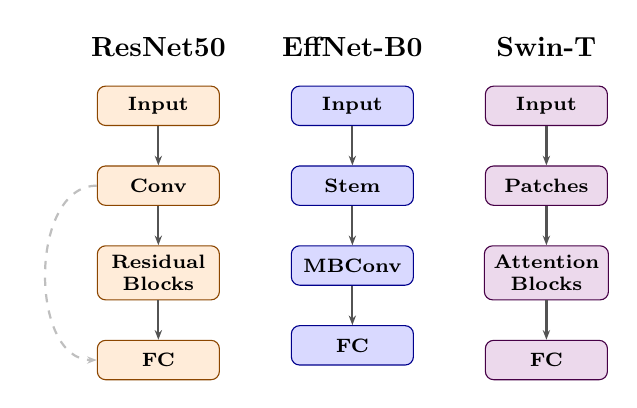
\begin{tikzpicture}[
    node distance=0.5cm and 0.9cm,
    every node/.style={align=center, font=\small}
]
  % ResNet50
  \node[pbox=orange] (r1) {Input};
  \node[pbox=orange, below=of r1] (r2) {Conv};
  \node[pbox=orange, below=of r2] (r3) {Residual\\Blocks};
  \node[pbox=orange, below=of r3] (r4) {FC};
  \draw[parr](r1)--(r2);\draw[parr](r2)--(r3);\draw[parr](r3)--(r4);
  \draw[skarr](r2.west) to[out=180,in=180] (r4.west);
  % EffNet-B0
  \node[pbox=blue, right=of r1] (e1) {Input};
  \node[pbox=blue, below=of e1] (e2) {Stem};
  \node[pbox=blue, below=of e2] (e3) {MBConv};
  \node[pbox=blue, below=of e3] (e4) {FC};
  \draw[parr](e1)--(e2);\draw[parr](e2)--(e3);\draw[parr](e3)--(e4);
  % Swin-T
  \node[pbox=violet, right=of e1] (s1) {Input};
  \node[pbox=violet, below=of s1] (s2) {Patches};
  \node[pbox=violet, below=of s2] (s3) {Attention\\Blocks};
  \node[pbox=violet, below=of s3] (s4) {FC};
  \draw[parr](s1)--(s2);\draw[parr](s2)--(s3);\draw[parr](s3)--(s4);
  % titles
  \node[above=0.25cm of r1, font=\bfseries] {ResNet50};
  \node[above=0.25cm of e1, font=\bfseries] {EffNet-B0};
  \node[above=0.25cm of s1, font=\bfseries] {Swin-T};
\end{tikzpicture}
\caption{Simplified backbone architectures used in the framework.}
\label{fig:backbones}
\end{figure}

Figure~\ref{fig:backbones} illustrates the main processing stages of the three backbones. ResNet50 uses residual blocks to learn deep convolutional representations; EfficientNet-B0 uses mobile inverted bottleneck blocks and compound scaling; and Swin Transformer partitions feature maps into local windows and applies shifted-window attention. The figure is a conceptual summary rather than a layer-by-layer specification.

\subsection{ResNet50}

ResNet50 \cite{he2016deep} is a CNN with residual connections, which allow very deep networks to be trained without vanishing gradients. Through skip connections, the model retains characteristics learned at earlier stages. Each bottleneck block computes:
\begin{equation}
    \mathbf{y} = \mathcal{F}(\mathbf{x},\{W_i\}) + W_s\mathbf{x}
    \label{eq:resnet}
\end{equation}
where $\mathbf{x}$ is the input, $\mathcal{F}$ is the residual function, $W_s$ denotes the shortcut projection, and $\mathbf{y}$ is the output. Four stages of 3, 4, 6, and 3 bottleneck blocks are followed by global average pooling and a task-specific linear head:
\begin{equation}
    \hat{y} = \mathrm{softmax}\left(W_{\mathrm{fc}} \cdot \mathrm{GAP}(\mathbf{A}^L) + b_{\mathrm{fc}}\right)
\end{equation}
where $\mathbf{A}^L$ is the final feature map, $\mathrm{GAP}$ denotes global average pooling, $W_{\mathrm{fc}}$ and $b_{\mathrm{fc}}$ are the classifier weights and bias, and $\hat{y}$ is the predicted output.

\subsection{EfficientNet-B0}

EfficientNet-B0 \cite{tan2019efficientnet} is the base model of a family obtained by scaling a network systematically rather than along a single dimension. Depth $d$, width $w$, and resolution $r$ are scaled jointly using a compound coefficient $\phi$:
\begin{equation}
    d = \alpha^\phi,\quad w = \beta^\phi,\quad r = \gamma^\phi,\quad
    \alpha \cdot \beta^2 \cdot \gamma^2 \approx 2
    \label{eq:effnet}
\end{equation}
where $\alpha, \beta, \gamma$ are scaling constants and $\phi$ controls model size.

EfficientNet uses mobile inverted bottleneck convolutions with Squeeze-and-Excitation~\cite{hu2018senet}, in which channel-wise attention is computed as:
\begin{equation}
    \mathbf{s} = \sigma(W_2\,\delta(W_1\,\mathrm{GAP}(\mathbf{z}))), \quad
    \hat{\mathbf{z}} = \mathbf{s} \odot \mathbf{z}
    \label{eq:se}
\end{equation}
where $\mathbf{z}$ is the input feature, $\mathrm{GAP}$ denotes global average pooling, $W_1, W_2$ are learnable weights, $\delta$ and $\sigma$ are activation functions, and $\mathbf{s}$ represents channel attention. This channel-wise recalibration is useful for cytological images, where nuclei and cytoplasm occupy spatially separable but morphologically distinct regions.

\subsection{Swin Transformer}

Swin Transformer \cite{liu2021swin} is based on self-attention rather than convolution. It splits the input image into patches and, instead of computing attention globally, partitions the feature map into $M\times M$ local windows and computes multi-head self-attention within each, reducing complexity from quadratic to linear in image resolution:
\begin{equation}
    \Omega(\mathrm{W\text{-}MSA}) = 4HWC^2 + 2M^2HWC
    \label{eq:wmsa}
\end{equation}
where $H$ and $W$ denote the spatial dimensions, $C$ is the channel dimension, and $M$ is the window size.

Attention within each window uses a learnable relative position bias:
\begin{equation}
    \mathrm{Attn}(Q,K,V) = \mathrm{softmax}\!\left(\frac{QK^\top}{\sqrt{d_k}} + B\right)V
    \label{eq:attn}
\end{equation}
where $Q$, $K$, and $V$ are the query, key, and value matrices, $d_k$ is the key dimension, and $B$ denotes the relative position bias. Shifting the windows between successive layers allows the model to learn both local and global dependencies. The hierarchical four-stage design produces feature maps from $H/4$ to $H/32$, encoding cues at multiple morphological scales simultaneously --- an expected benefit given that nuclear texture, perinuclear halo geometry, and cytoplasmic area operate at different physical scales.

\begin{table}[ht]
\centering
\caption{Experimental Environment}
\label{tab:environment}
\begin{tabular}{|l|l|}
\hline
\textbf{Component} & \textbf{Specification} \\ \hline
Operating System & Windows 11 \\ \hline
Python Version & Python 3.11 \\ \hline
Deep Learning Framework & PyTorch 2.x \\ \hline
IDE & VS Code  \\ \hline
Model Architectures & EfficientNet-B0, ResNet50, Swin Transformer \\ \hline
XAI Technique & Grad-CAM++ \\ \hline
Frontend & React.js \\ \hline
Backend & FastAPI \\ \hline
Visualization & Streamlit Dashboard \\ \hline
Datasets & SIPaKMeD, Herlev \\ \hline
GPU (training and evaluation) & NVIDIA RTX 3050 \\ \hline
GPU (efficiency benchmark, Table~\ref{tab:efficiency}) & NVIDIA A100 \\ \hline
RAM & 16 GB \\ \hline
\end{tabular}
\end{table}

%------------------------------------------------------------------
\section{Training Configuration}
\label{sec:training}

Model training uses cross-entropy loss with label smoothing ($\varepsilon=0.1$)~\cite{szegedy2016rethinking}:
\begin{equation}
    \mathcal{L} =
    -\frac{1}{N}\sum_{i,k}\tilde{y}_{ik}\log \hat{y}_{ik}, \quad
    \tilde{y}_{ik} = (1 - \varepsilon)y_{ik} + \frac{\varepsilon}{K}
    \label{eq:loss}
\end{equation}
where $\hat{y}_{ik}$ is the predicted probability, $y_{ik}$ is the ground truth label, $K$ is the number of classes, and $\varepsilon$ is the smoothing factor.

Optimization is performed using AdamW~\cite{loshchilov2019adamw} with $\beta_1=0.9$, $\beta_2=0.999$, and weight decay $10^{-4}$.

A cosine annealing schedule~\cite{loshchilov2017sgdr} is used for learning rate decay:
\begin{equation}
    \eta_t = \eta_{\min} + \tfrac{1}{2}(\eta_{\max} - \eta_{\min})
    \left(1 + \cos\!\left(\frac{T_{\mathrm{cur}}}{T_{\mathrm{max}}}\pi\right)\right)
    \label{eq:cosine}
\end{equation}
where $\eta_t$ is the learning rate at step $t$, and $T_{\mathrm{cur}}$, $T_{\mathrm{max}}$ denote the current and total training steps. A five-epoch warm-up period stabilizes early training. Initial learning rates reflect the differing sensitivities of the models: the CNN backbones start at $\eta_0=3\times10^{-4}$ and Swin-T at $1\times10^{-4}$, because transformers are more sensitive to large early updates.

Training proceeds in two stages. In the first, the backbone is frozen and only the classification head is trained. In the second, the whole model is fine-tuned with layer-wise learning-rate decay $\eta^{(l)}=\eta_0\cdot0.75^{L-l}$.

Overfitting is controlled with dropout ($p=0.3$) and stochastic depth (maximum rate 0.2 for Swin-T). Models are trained for up to 100 epochs with early stopping (patience 15).

Model efficiency (parameters, FLOPs, and single-image inference latency, Table~\ref{tab:efficiency}) was benchmarked separately on an NVIDIA A100 GPU; all training and accuracy evaluation were performed on the RTX 3050 system described in Table~\ref{tab:environment}.

%------------------------------------------------------------------
\subsection{Performance Metrics}
The models are evaluated using accuracy, precision, recall (sensitivity), specificity, and F1-score. For binary classification, the metrics are computed from the numbers of true positives (TP), true negatives (TN), false positives (FP), and false negatives (FN):
\begin{equation}
    \mathrm{Accuracy}=\frac{TP+TN}{TP+TN+FP+FN}
    \label{eq:accuracy}
\end{equation}
\begin{equation}
    \mathrm{Precision}=\frac{TP}{TP+FP},\qquad
    \mathrm{Recall}=\frac{TP}{TP+FN}
    \label{eq:precision_recall}
\end{equation}
\begin{equation}
    \mathrm{Specificity}=\frac{TN}{TN+FP},\qquad
    \mathrm{F1}=2\frac{\mathrm{Precision}\times\mathrm{Recall}}
    {\mathrm{Precision}+\mathrm{Recall}}
    \label{eq:specificity_f1}
\end{equation}
Here, TP is the number of positive samples correctly classified as positive, TN the number of negative samples correctly classified as negative, FP the number of negative samples incorrectly classified as positive, and FN the number of positive samples incorrectly classified as negative. Precision is the proportion of predicted positives that are correct, recall the proportion of actual positives detected, and specificity the proportion of actual negatives correctly identified. The F1-score is the harmonic mean of precision and recall. For multiclass classification, these measures are computed per class in a one-versus-rest manner, and macro-averaged values are the unweighted mean across classes. AUC denotes the area under the receiver operating characteristic curve, and MCC the Matthews correlation coefficient.

%------------------------------------------------------------------
\section{Results}
\label{sec:results}

\subsection{Multiclass Classification}

Swin Transformer attains the best multiclass performance of the three individual models, with an accuracy of 96.8\% and the highest precision, recall, and F1-score (Table~\ref{tab:multiclass}). EfficientNet-B0 scores lower but uses far fewer parameters than Swin Transformer (Table~\ref{tab:efficiency}). ResNet50 performs well but trails the other two models. These results suggest that an architecture that captures multi-scale features and global context, as Swin Transformer does, is advantageous for fine-grained cervical cell classification. The three-model soft-voting ensemble reaches 97.1\% multiclass accuracy (Fig.~\ref{fig:accbar}).

\begin{table}[t]
\caption{Multiclass Test-Set Performance (in-distribution, cell-level split)}
\label{tab:multiclass}
\centering
\setlength{\tabcolsep}{3.5pt}
\begin{tabular}{lcccccc}
\toprule
\textbf{Model} & \textbf{Acc\%} & \textbf{P\%} & \textbf{R\%} & \textbf{F1\%} & \textbf{AUC} & \textbf{MCC}\\
\midrule
ResNet50        & 93.5 & 93.0 & 93.2 & 93.1 & 0.971 & 0.919\\
EfficientNet-B0 & 95.2 & 94.8 & 95.0 & 94.9 & 0.981 & 0.940\\
Swin-T          & \textbf{96.8} & \textbf{96.4} & \textbf{96.6} & \textbf{96.5} & \textbf{0.987} & \textbf{0.962}\\
\bottomrule
\end{tabular}
\begin{flushleft}
\footnotesize \textit{Note:} Acc = accuracy, P = precision, R = recall, F1 = F1-score, AUC = area under the ROC curve, MCC = Matthews correlation coefficient.
\end{flushleft}
\end{table}

\subsection{Binary Classification}

For binary classification, all models exceed 97\% accuracy, and the differences between them are small (Table~\ref{tab:binary}). The gap between the best and worst backbone narrows from 3.3 percentage points in the multiclass task to 1.4 points in the binary task: as the easier task approaches saturation, the choice of backbone matters less than it does for fine-grained subtyping. The ensemble reaches 98.7\% binary accuracy (Fig.~\ref{fig:accbar}).

\begin{table}[t]
\caption{Binary Classification Performance (in-distribution, cell-level split)}
\label{tab:binary}
\centering
\setlength{\tabcolsep}{3.5pt}
\begin{tabular}{lccccc}
\toprule
\textbf{Model} & \textbf{Acc\%} & \textbf{Sens.} & \textbf{Spec.} & \textbf{F1\%} & \textbf{AUC}\\
\midrule
ResNet50        & 97.1 & 0.968 & 0.975 & 97.0 & 0.987\\
EfficientNet-B0 & 97.9 & 0.977 & 0.981 & 97.8 & 0.991\\
Swin-T          & \textbf{98.5} & \textbf{0.984} & \textbf{0.986} & \textbf{98.4} & \textbf{0.994}\\
\bottomrule
\end{tabular}
\begin{flushleft}
\footnotesize \textit{Note:} Sens. = sensitivity, Spec. = specificity, F1 = F1-score, AUC = area under the ROC curve.
\end{flushleft}
\end{table}

\subsection{Confusion Analysis and Training Dynamics}

The most frequent misclassification across all models is Koilocytotic predicted as Dyskeratotic (4.1\% for Swin-T and higher for the other two), which is unsurprising because both categories involve nuclear abnormalities and the visual distinction is subtle even for experienced readers. Parabasal cells achieved perfect recall under Swin-T, largely because their small, dark, round nuclei are morphologically unlike any other class in either dataset. All models converged within 72 epochs; final validation losses were 0.108, 0.159, and 0.213 for Swin-T, EfficientNet-B0, and ResNet50 respectively, consistent with their accuracy ranking.

% ---- Accuracy bar chart ----
\begin{figure}[t]
\centering
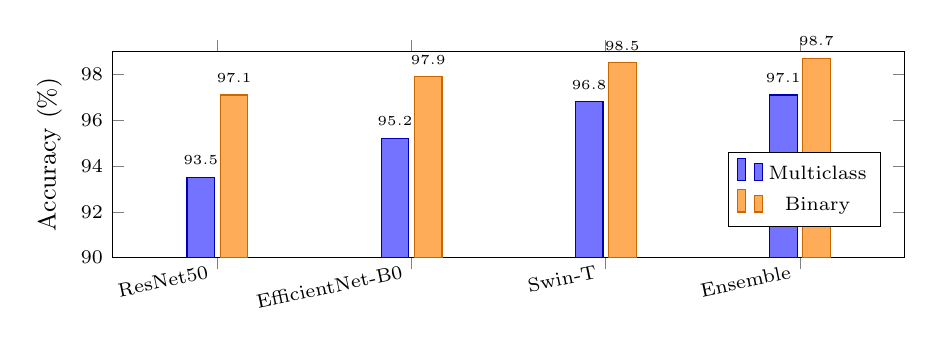
\begin{tikzpicture}
\begin{axis}[
  ybar,
  bar width=10pt,
  width=0.96\columnwidth,
  height=4.2cm,
  ylabel={\small Accuracy (\%)},
  ylabel style={font=\small},
  symbolic x coords={ResNet50, EfficientNet-B0, Swin-T, Ensemble},
  xtick=data,
  x tick label style={font=\scriptsize, rotate=12, anchor=east},
  ymin=90, ymax=99,
  ytick={90,92,94,96,98},
  yticklabel style={font=\scriptsize},
  legend style={font=\scriptsize, at={(0.97,0.15)},
                anchor=south east, legend columns=1},
  enlarge x limits=0.18,
  nodes near coords,
  nodes near coords style={font=\tiny, anchor=south},
  every node near coord/.append style={yshift=1pt},
]
% Multiclass bars
\addplot[fill=blue!55, draw=blue!70!black]
  coordinates {(ResNet50,93.5)(EfficientNet-B0,95.2)(Swin-T,96.8)(Ensemble,97.1)};
% Binary bars
\addplot[fill=orange!65, draw=orange!80!black]
  coordinates {(ResNet50,97.1)(EfficientNet-B0,97.9)(Swin-T,98.5)(Ensemble,98.7)};
\legend{Multiclass, Binary}
\end{axis}
\end{tikzpicture}
\caption{Multiclass and binary accuracy of the individual models and of the three-model soft-voting ensemble (ResNet50 + EfficientNet-B0 + Swin-T).}
\label{fig:accbar}
\end{figure}

\subsection{Cross-Dataset Generalization}
\label{sec:cross}

Table~\ref{tab:cross} reports two kinds of experiment. In the cross-dataset rows, a model is trained on one dataset and tested on the entire other dataset, which it has never seen. Accuracy drops to 68.4--80.2\%, showing that models trained on a single source do not transfer well. The drop can be attributed to differences in staining, acquisition equipment, and image resolution between the two collections. Swin-T transfers best in both directions.

In the in-distribution rows, a model trained on the combined training split is tested on the held-out test portion of each source. Because cells from that source were also present in training, these rows are not cross-dataset results: they show that a single model can fit both sources simultaneously (88.6--95.7\%), not that combined training generalizes to an unseen distribution. Testing generalization to a truly unseen source would require a third dataset, such as CRIC \cite{rezende2021cric}, which we leave to future work.

\begin{table}[t]
\caption{Cross-Dataset and In-Distribution Accuracy (\%). ``Combined'' rows are evaluated on the held-out test portion of the named source, whose other images were used in training; they are in-distribution, not cross-dataset.}
\label{tab:cross}
\centering
\setlength{\tabcolsep}{3.5pt}
\begin{tabular}{llccc}
\toprule
\textbf{Train $\to$ Test} & \textbf{Setting} & \textbf{ResNet50} & \textbf{EfficientNet} & \textbf{Swin-T}\\
\midrule
SIPaKMeD $\to$ Herlev                   & Cross-dataset   & 71.3 & 76.8 & 80.2\\
Herlev $\to$ SIPaKMeD                   & Cross-dataset   & 68.4 & 74.1 & 77.9\\
\midrule
Combined $\to$ Herlev (held-out test)   & In-distribution & 88.6 & 91.2 & 93.4\\
Combined $\to$ SIPaKMeD (held-out test) & In-distribution & 91.8 & 93.9 & 95.7\\
\bottomrule
\end{tabular}
\end{table}

%------------------------------------------------------------------
\section{Explainable AI and System Architecture}
\label{sec:xai}

\subsection{Grad-CAM++ Formulation}

To make predictions transparent, Grad-CAM++ \cite{chattopadhay2018} is used to produce a visual explanation of each prediction by highlighting the image regions associated with the predicted class. Grad-CAM++ generalizes Grad-CAM \cite{selvaraju2017gradcam}, whose formulation is given first. For a target class $c$, Grad-CAM spatially averages the gradients of the class score $y^c$ with respect to the final feature map $\mathbf{A}^k$:
\begin{equation}
    \alpha_k^c = \frac{1}{Z}\sum_i\sum_j
    \frac{\partial y^c}{\partial A^k_{ij}}, \quad Z = u \times v
    \label{eq:gradcam_w}
\end{equation}
where $A^k_{ij}$ is the activation at spatial location $(i,j)$ in feature map $k$, $y^c$ is the score for target class $c$, $\alpha_k^c$ is the importance weight assigned to feature map $k$, and $Z=u\times v$ is the number of spatial locations in a feature map of height $u$ and width $v$.

A weighted sum followed by ReLU gives the saliency map:
\begin{equation}
    L^c = \mathrm{ReLU}\!\left(\sum_k \alpha_k^c \mathbf{A}^k\right)
    \label{eq:gradcam}
\end{equation}
where $L^c$ is the class-specific localization map, $k$ indexes the feature maps, and ReLU suppresses negative contributions.

Grad-CAM++, the method used throughout this work, replaces the uniform average in Eq.~\ref{eq:gradcam_w} with pixel-wise weights derived from higher-order gradients, which improves localization when several relevant regions are present:
\begin{equation}
    \alpha_k^{c,++} = \frac{{\partial^2 y^c}/{\partial(A^k_{ij})^2}}
    {2\,{\partial^2 y^c}/{\partial(A^k_{ij})^2}
    + \sum_{a,b} A^k_{ab}\,{\partial^3 y^c}/{\partial(A^k_{ij})^3}}
    \label{eq:gradcampp}
\end{equation}
where $\alpha_k^{c,++}$ denotes the Grad-CAM++ importance weight associated with feature map $k$ and target class $c$, and the spatial indices $(i,j)$ and $(a,b)$ refer to locations within the feature map. The resulting map (Eq.~\ref{eq:gradcam} with these weights) is upsampled bilinearly to $224 \times 224$ and overlaid on the input cell image (Fig.~\ref{fig:gradcam}).

\begin{figure}[t]
    \centering
    % Replace with a Grad-CAM++ heatmap computed on ONE single-cell test crop
    % (input crop on the left, overlay on the right).
    \includegraphics[width=0.8\linewidth]{gradcam_single_cell.png}
    \caption{Grad-CAM++ explanation for a single classified cell crop from the test set (Swin-T). Left: input cell image; right: heatmap overlay. Warmer colors mark the regions that contributed most to the predicted class.}
    \label{fig:gradcampp}
\end{figure}

\begin{figure*}[t]
\centering
\resizebox{0.98\textwidth}{!}{%
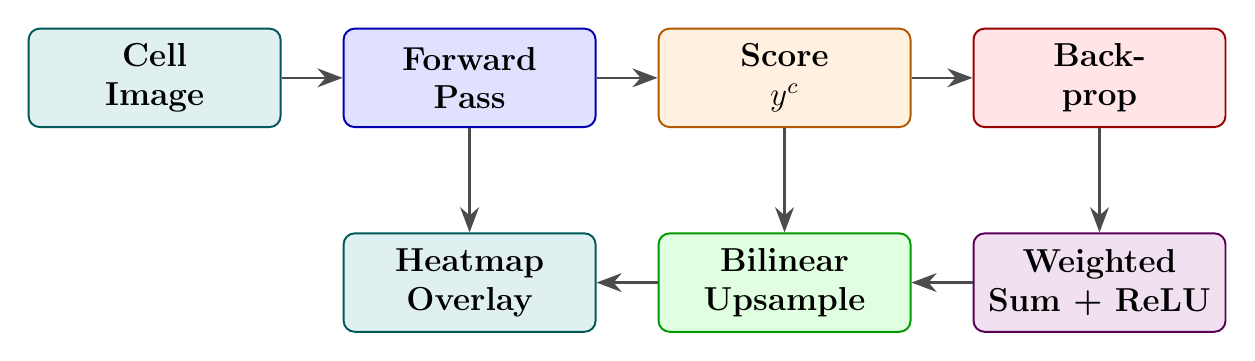
\begin{tikzpicture}[
    arrow/.style={-{Stealth[length=3.2mm]}, thick, draw=black!70},
    box/.style={
        draw,
        rounded corners=4pt,
        minimum width=3.2cm,
        minimum height=1.25cm,
        align=center,
        font=\bfseries\large,
        line width=0.7pt
    }
]

% -------- Top row --------
\node[box, fill=teal!12, draw=teal!70!black]   (img)   at (0, 2.4) {Cell\\Image};
\node[box, fill=blue!12, draw=blue!70!black]    (fwd)   at (4.0, 2.4) {Forward\\Pass};
\node[box, fill=orange!12, draw=orange!70!black] (sc)    at (8.0, 2.4) {Score\\$y^c$};
\node[box, fill=red!10, draw=red!60!black]      (bp)    at (12.0, 2.4) {Back-\\prop};

% -------- Bottom row --------
\node[box, fill=teal!12, draw=teal!70!black]    (feat)  at (4.0, -0.2) {Heatmap\\Overlay};
\node[box, fill=green!12, draw=green!60!black]   (up)    at (8.0, -0.2) {Bilinear\\Upsample};
\node[box, fill=violet!12, draw=violet!70!black] (wsum)  at (12.0, -0.2) {Weighted\\Sum + ReLU};

% -------- Top flow --------
\draw[arrow] (img) -- (fwd);
\draw[arrow] (fwd) -- (sc);
\draw[arrow] (sc) -- (bp);

% -------- Vertical connections --------
\draw[arrow] (fwd) -- (feat);
\draw[arrow] (sc) -- (up);
\draw[arrow] (bp) -- (wsum);

% -------- Bottom flow --------
\draw[arrow] (wsum) -- (up);
\draw[arrow] (up) -- (feat);

\end{tikzpicture}%
}
\caption{Grad-CAM++ computation: backpropagated gradients weight the feature maps, and the resulting saliency map is upsampled and overlaid on the cell image.}
\label{fig:gradcam}
\end{figure*}

\subsection{Qualitative Findings}

Qualitatively, the highlighted regions tend to coincide with cytologically meaningful features such as abnormal nuclear shape and chromatin. For abnormal cells, attention concentrates mainly on the nucleus and the perinuclear region. Swin Transformer produces more focused maps than ResNet50, which more often highlights irrelevant background. These observations are qualitative and have not been validated against cytopathologist annotations.

\subsection{End-to-End Pipeline}

The system follows a structured pipeline: image acquisition and preprocessing, nuclear segmentation with a U-Net trained on MoNuSeg, and classification by three complementary backbones --- ResNet50, EfficientNet-B0, and Swin Transformer --- whose predictions are combined by soft voting:
\begin{equation}
    \hat{P}(y=k \mid x)=\frac{1}{M}\sum_{m=1}^{M}\hat{P}_m(y=k \mid x), \qquad M=3
    \label{eq:ensemble}
\end{equation}
where $\hat{P}_m(y=k \mid x)$ is the softmax probability of class $k$ from backbone $m$. The prediction is combined with cytological feature scores and mapped to a Bethesda category (Section~\ref{sec:bethesda}, Eq.~\ref{eq:fusion}) and accompanied by a Grad-CAM++ explanation.

Table~\ref{tab:efficiency} compares computational costs. Because the ensemble runs all three backbones, its parameter count and FLOPs are the sums of those of the individual models. EfficientNet-B0, with the lowest latency and parameter count, is best suited to edge deployment, whereas the ensemble gives the highest accuracy at roughly four times the latency of EfficientNet-B0 alone.

\begin{table}[t]
\caption{Model Efficiency (benchmarked on an NVIDIA A100, batch size 1). The ensemble runs all three backbones.}
\label{tab:efficiency}
\centering
\begin{tabular}{lcccc}
\toprule
\textbf{Model} & \textbf{Params (M)} & \textbf{FLOPs (G)} & \textbf{Lat.\ (ms)} & \textbf{Acc\%}\\
\midrule
ResNet50        & 25.6 & 4.1 & --   & 93.5\\
EfficientNet-B0 & 5.3  & 0.4 & 8.7  & 95.2\\
Swin-T          & 28.3 & 4.5 & 18.6 & 96.8\\
Ensemble (all three) & 59.2 & 9.0 & 39.6 & 97.1\\
\bottomrule
\end{tabular}
\end{table}

%------------------------------------------------------------------
\section{Conclusion and Future Work}
\label{sec:conclusion}

This study shows that deep learning, and Swin Transformer in particular, is well suited to classifying cervical cells from Pap smear images, and that EfficientNet-B0 offers a good balance between accuracy and efficiency for resource-limited settings. Five conclusions can be drawn. First, Swin Transformer is the best individual classifier, with a multiclass accuracy of 96.8\% and a macro-AUC of 0.987, and the three-model ensemble raises accuracy to 97.1\%. Second, models trained on a single dataset transfer poorly to the other (68--80\% accuracy), which confirms a substantial domain gap between SIPaKMeD and Herlev; training on the combined data allows one model to perform well on held-out images from both sources, although this is an in-distribution result rather than evidence of generalization to unseen sources. Third, Grad-CAM++ maps tend to highlight nuclear and perinuclear regions that cytopathologists also use, which supports interpretability, although this agreement has not yet been quantified. Fourth, the U-Net segmentation stage provides a nuclear-focused input to the classifiers, but its segmentation quality on cervical cytology and its effect on accuracy remain to be measured. Lastly, reporting outputs as NILM, ASC-US, LSIL, HSIL, and SCC through the fused clinical score gives cytopathologists a familiar frame of reference; the mapping is not a substitute for Bethesda reporting by a cytopathologist.

Future work will address the limitations identified above: a slide- or source-image-level grouped split to remove possible leakage between training and test cells; Dice-based evaluation of the U-Net against the nucleus annotations available in SIPaKMeD and Herlev, together with an ablation of the segmentation stage; and external validation on a third dataset with native Bethesda labels, such as CRIC \cite{rezende2021cric} or HiCervix \cite{cai2024hicervix}, which would also allow the score intervals, including the ASC-US band, to be evaluated against native Bethesda labels. Further directions include enlarging the training set, whole-slide image (WSI) classification \cite{dang2023wsi} with patch-based inference and attention pooling \cite{ilse2018attention}, federated learning across institutions to protect patient privacy \cite{rieke2020federated}, and prospective clinical validation through reader studies. Clinical reliability could also be improved by uncertainty-aware modelling, for example Monte Carlo dropout \cite{gal2016dropout}, to produce outputs such as ``HSIL (confidence: 62\%) -- manual review recommended''.

\section*{Acknowledgement}
The authors sincerely thank Dr.~Vijayalakshmi Ramshankar and Dr.~Srinidhi Sairaman from Cancer Biology and Molecular Diagnostics, Cancer Institute WIA, Adyar, Chennai, for their support and guidance on cervical cancer diagnosis.

%------------------------------------------------------------------
\begin{thebibliography}{00}

\bibitem{who2022}
World Health Organization: Cervical Cancer. WHO Fact Sheets (Feb. 2022)

\bibitem{arbyn2010}
Arbyn, M., et al.: European guidelines for quality assurance in cervical cancer screening. Ann. Oncology \textbf{21}(suppl. 3), iii448--iii458 (2010)

\bibitem{he2016deep}
He, K., Zhang, X., Ren, S., Sun, J.: Deep residual learning for image recognition. In: Proc. IEEE CVPR, pp. 770--778 (2016)

\bibitem{tan2019efficientnet}
Tan, M., Le, Q.: EfficientNet: Rethinking model scaling for convolutional neural networks. In: Proc. ICML, pp. 6105--6114 (2019)

\bibitem{liu2021swin}
Liu, Z., et al.: Swin Transformer: Hierarchical vision transformer using shifted windows. In: Proc. IEEE ICCV, pp. 10012--10022 (2021)

\bibitem{plissiti2018sipakmed}
Plissiti, M.E., Dimitrakopoulos, P., Sfikas, G., Nikou, C., Krikoni, O., Charchanti, A.: SIPaKMeD: A new dataset for feature and image based classification of normal and pathological cervical cells in Pap smear images. In: Proc. 25th IEEE International Conference on Image Processing (ICIP), pp. 3144--3148 (2018)

\bibitem{jantzen2005}
Jantzen, J., Norup, J., Dounias, G., Bjerregaard, B.: Pap-smear benchmark data for pattern classification. In: Proc. Nature Inspired Smart Information Systems (NiSIS), pp. 1--9 (2005)

\bibitem{selvaraju2017gradcam}
Selvaraju, R.R., et al.: Grad-CAM: Visual explanations from deep networks via gradient-based localization. In: Proc. IEEE ICCV, pp. 618--626 (2017)

\bibitem{zhang2017deeppap}
Zhang, L., Lu, L., Nogues, I., Summers, R.M., Liu, S., Yao, J.: DeepPap: Deep convolutional networks for cervical cell classification. IEEE J. Biomed. Health Inform. \textbf{21}(6), 1633--1643 (2017)

\bibitem{lin2019}
Lin, H., Hu, Y., Chen, S., Yao, J., Zhang, L.: Fine-grained classification of cervical cells using morphological and appearance based convolutional neural networks. IEEE Access \textbf{7}, 71541--71549 (2019)

\bibitem{rahaman2020}
Rahaman, M.M., Li, C., Wu, X., Yao, Y., Hu, Z., Jiang, T., Li, X., Qi, S.: A survey for cervical cytopathology image analysis using deep learning. IEEE Access \textbf{8}, 61687--61710 (2020)

\bibitem{chen2022hipt}
Chen, R.J., Chen, C., Li, Y., Chen, T.Y., Trister, A.D., Krishnan, R.G., Mahmood, F.: Scaling vision transformers to gigapixel images via hierarchical self-supervised learning. In: Proc. IEEE/CVF CVPR, pp. 16144--16155 (2022)

\bibitem{rezende2021cric}
Rezende, M.T., et al.: Cric searchable image database as a public platform for conventional pap smear cytology data. Scientific Data \textbf{8}, 151 (2021)

\bibitem{cai2024hicervix}
Cai, D., et al.: HiCervix: An extensive hierarchical dataset and benchmark for cervical cytology classification. IEEE Trans. Med. Imaging \textbf{43}(12), 4344--4355 (2024)

\bibitem{liu2022cvmcervix}
Liu, W., Li, C., et al.: CVM-Cervix: A hybrid cervical Pap-smear image classification framework using CNN, visual transformer and multilayer perceptron. Pattern Recognition \textbf{130}, 108829 (2022)

\bibitem{pacal2024maxcervixt}
Pacal, I.: MaxCerVixT: A novel lightweight vision transformer-based approach for precise cervical cancer detection. Knowledge-Based Systems \textbf{289}, 111482 (2024)

\bibitem{stacke2021domainshift}
Stacke, K., Eilertsen, G., Unger, J., Lundstr\"om, C.: Measuring domain shift for deep learning in histopathology. IEEE J. Biomed. Health Inform. \textbf{25}(2), 325--336 (2021)

\bibitem{chattopadhay2018}
Chattopadhay, A., et al.: Grad-CAM++: Generalized gradient-based visual explanations for deep convolutional networks. In: Proc. IEEE WACV, pp. 839--847 (2018)

\bibitem{esteva2017}
Esteva, A., et al.: Dermatologist-level classification of skin cancer with deep neural networks. Nature \textbf{542}, 115--118 (2017)

\bibitem{rajpurkar2017}
Rajpurkar, P., et al.: CheXNet: Radiologist-level pneumonia detection on chest X-rays with deep learning. arXiv:1711.05225 (2017)

\bibitem{zhang2018mixup}
Zhang, H., et al.: mixup: Beyond empirical risk minimization. In: Proc. ICLR (2018)

\bibitem{ronneberger2015unet}
Ronneberger, O., Fischer, P., Brox, T.: U-Net: Convolutional networks for biomedical image segmentation. In: Medical Image Computing and Computer-Assisted Intervention (MICCAI 2015), LNCS, vol. 9351, pp. 234--241. Springer (2015)

\bibitem{kumar2017monuseg}
Kumar, N., Verma, R., Sharma, S., Bhargava, S., Vahadane, A., Sethi, A.: A multi-organ nucleus segmentation challenge. In: Proc. IEEE International Symposium on Biomedical Imaging (ISBI), pp. 1380--1384 (2017)

\bibitem{gal2016dropout}
Gal, Y., Ghahramani, Z.: Dropout as a Bayesian approximation. In: Proc. ICML, pp. 1050--1059 (2016)

\bibitem{hu2018senet}
Hu, J., Shen, L., Sun, G.: Squeeze-and-Excitation Networks. In: Proc. IEEE CVPR, pp. 7132--7141 (2018)

\bibitem{szegedy2016rethinking}
Szegedy, C., Vanhoucke, V., Ioffe, S., Shlens, J., Wojna, Z.: Rethinking the inception architecture for computer vision. In: Proc. IEEE CVPR, pp. 2818--2826 (2016)

\bibitem{loshchilov2019adamw}
Loshchilov, I., Hutter, F.: Decoupled weight decay regularization. In: Proc. ICLR (2019)

\bibitem{loshchilov2017sgdr}
Loshchilov, I., Hutter, F.: SGDR: Stochastic gradient descent with warm restarts. In: Proc. ICLR (2017)

\bibitem{dang2023wsi}
Dang, C., Qi, Z., Xu, T., Gu, M., Chen, J., Wu, J., Lin, Y., Qi, X.: Deep learning--powered whole slide image analysis in cancer pathology. Computers in Biology and Medicine \textbf{158}, 106773 (2023)

\bibitem{ilse2018attention}
Ilse, M., Tomczak, J.M., Welling, M.: Attention-based deep multiple instance learning. In: Proc. ICML, pp. 2132--2141 (2018)

\bibitem{rieke2020federated}
Rieke, N., et al.: The future of digital health with federated learning. NPJ Digital Med. \textbf{3}, 119 (2020)

\end{thebibliography}

\end{document}
